% !TeX spellcheck = fr_FR
\documentclass[../main.tex]{subfiles}

\begin{document}

\subsection{Données synthétiques}\label{ssec:synthResults}

Les modèles ont été entraînés sur des jeux de données synthétiques générées à partir d'un processus de Hawkes linéaire à noyau exponentiel, en utilisant la librairie \verb|tick| pour Python \cite{2017arXiv170703003B}.

Un premier indicateur pour voir si le modèle peut retrouver la structure d'un Hawkes est de regarder la distribution du nombre d'événements, au total $N_T$ et par type d'événement $N^k_T, k\in\llbracket 1,K\rrbracket$. Réaliser le graphe de l'intensité $\lambda_t$ pour une séquence d'événements simulée permet aussi de voir si les phénomènes d'auto-excitation sont reflétés.

On a utilisé deux jeux de données synthétiques, détaillés \autoref{tab:synthHawkesData}.

\begin{table}[h]
	\centering
	\begin{tabular}{@{}cccccccc}
		\toprule
		$K$ & \multicolumn{4}{c}{Paramètres} & Nb. moyen d'évts. & \multicolumn{2}{c}{Dataset} \\ \cmidrule(r){2-5}\cmidrule(r){7-8}
		    & $T$ & $\mu$ & $\alpha$ & $\beta$ & & Train & Test\\ \midrule
		1 & 3600 & 0.2 & 0.1 & 2.0 & $\approx 800$ & 4000 & 1000 \\ \midrule
		2 & 3600 & $(0.1, 0.1)^\intercal$ & $\begin{bmatrix}0.1 & 0.01\\0.01 &0.1\end{bmatrix}$ & 1.0 & $\approx 808$ & 3000 & 1000\\
		\bottomrule
	\end{tabular}
	\caption{Paramètres des données synthétiques.}\label{tab:synthHawkesData}
\end{table}

Des histogrammes des nombre d'événements entre $0$ et $T$ pour les modèles Decay-RNN et LSTM sont donnés \autoref{fig:1DlengthDistrib}.

\begin{figure}[ht]
	\begin{subfigure}{\linewidth}
		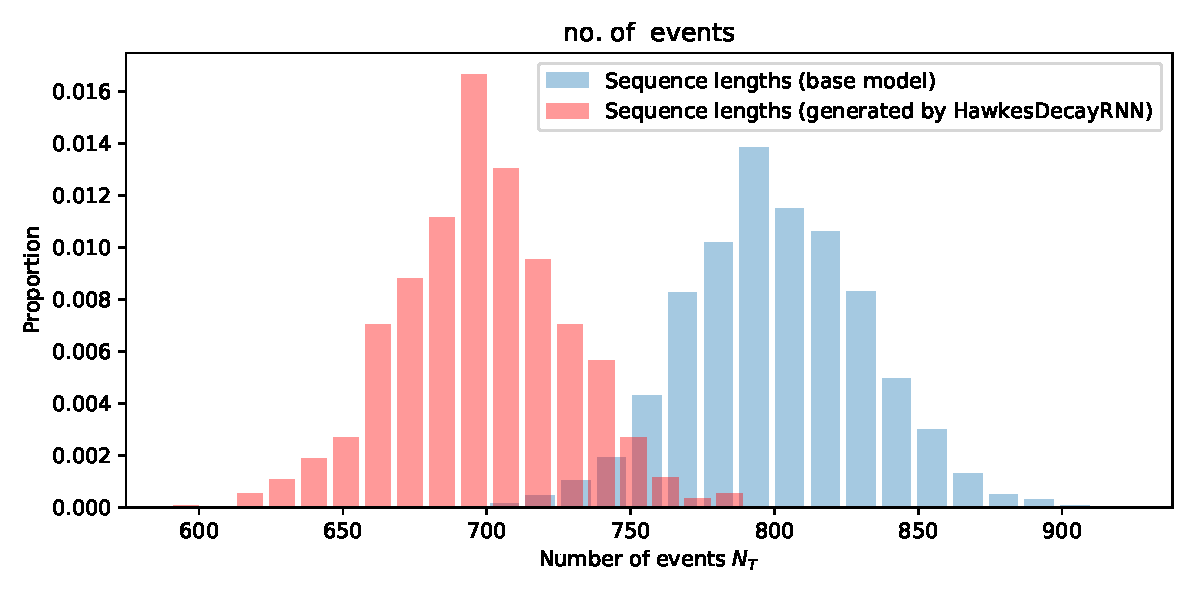
\includegraphics[width=\linewidth]{../results/length_distrib_HawkesDecayRNN-1d-hidden_64-20181206-234848.pdf}
		\caption{Distribution du nombre d'événements. Hawkes et Decay-RNN avec $K=1$, $D=64$ neurones cachés. Entraîné sur le jeu de données \autoref{tab:synthHawkesData}.}\label{fig:1DRNNlengthDistrib}
	\end{subfigure}
	\begin{subfigure}{\linewidth}
		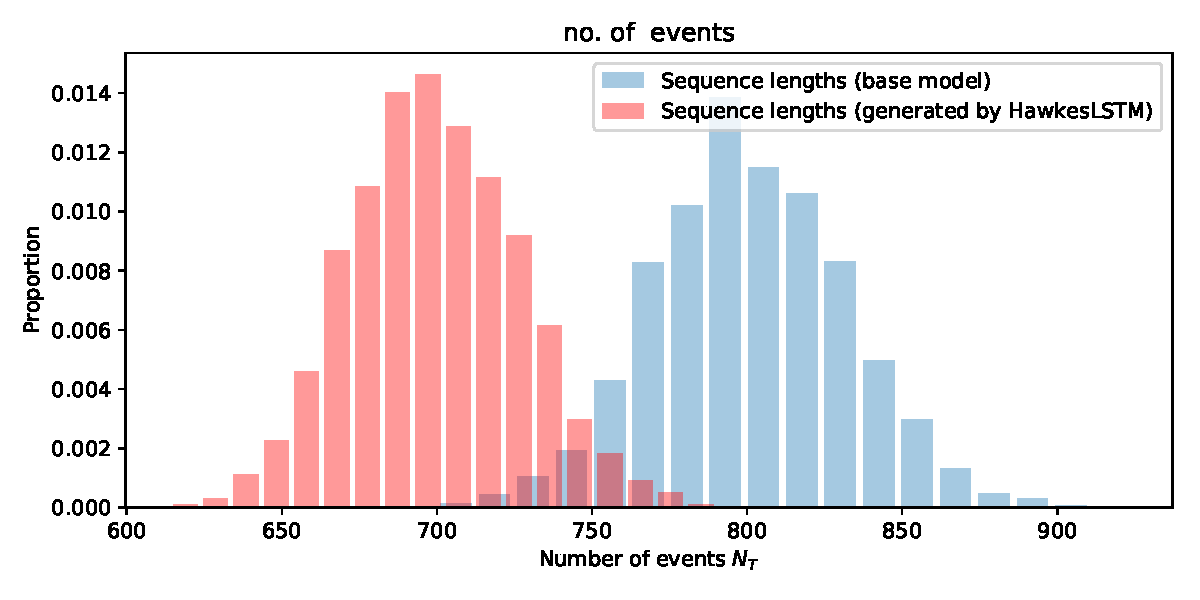
\includegraphics[width=\linewidth]{../results/length_distrib_HawkesLSTM-1d-hidden64-20181206-235311.pdf}
		\caption{Distribution du nombre d'événements. Hawkes et LSTM avec $K=1$, $D=64$ neurones cachés. Entraîné sur le jeu de données \autoref{tab:synthHawkesData}.}\label{fig:1DLSTMlengthDistrib}	
	\end{subfigure}
	\caption{Distributions des nombres d'événements pour les modèles Decay-RNN et LSTM entraînés sur le jeu de données synthétiques 1D.}\label{fig:1DlengthDistrib}
\end{figure}

Un autre critère d'évaluation que nous utilisons est l'erreur de prédiction sur les données de test, à la fois pour le temps d'arrivée du prochain événement et l'erreur sur son type (voir \autoref{fig:rmseSynthData}). Les résultats nous suggèrent que le LSTM souffrirait d'un problème de sur-ajustement par rapport au Decay-RNN. Globalement, les deux modèles ont une erreur assez élevée et n'arrivent pas à prédire correctement le type du prochain événement.

\begin{figure}[!ht]
	\includegraphics[width=\linewidth]{../results/intensity_HawkesDecayRNN_1d_hidden64_20181206-234848.pdf}
	\caption{Intensité d'un Decay-RNN univarié, entraîné sur les données 1D simulées à partir d'un Hawkes \autoref{tab:synthHawkesData}.}\label{fig:1DRNNintensityPlot}
\end{figure}

\begin{figure}[!ht]
	\centering
	\begin{subfigure}{0.8\linewidth}
		\centering
		\includegraphics[width=\linewidth]{../results/1D_Hawkes_Data_RMSE.pdf}
		\caption{RMSE, modèles Decay-RNN et LSTM. Données synthétiques Hawkes, $K=1$, $D=64$.}\label{fig:rmse1DhawkesData}	
	\end{subfigure}
	\begin{subfigure}{0.8\linewidth}
		\centering
		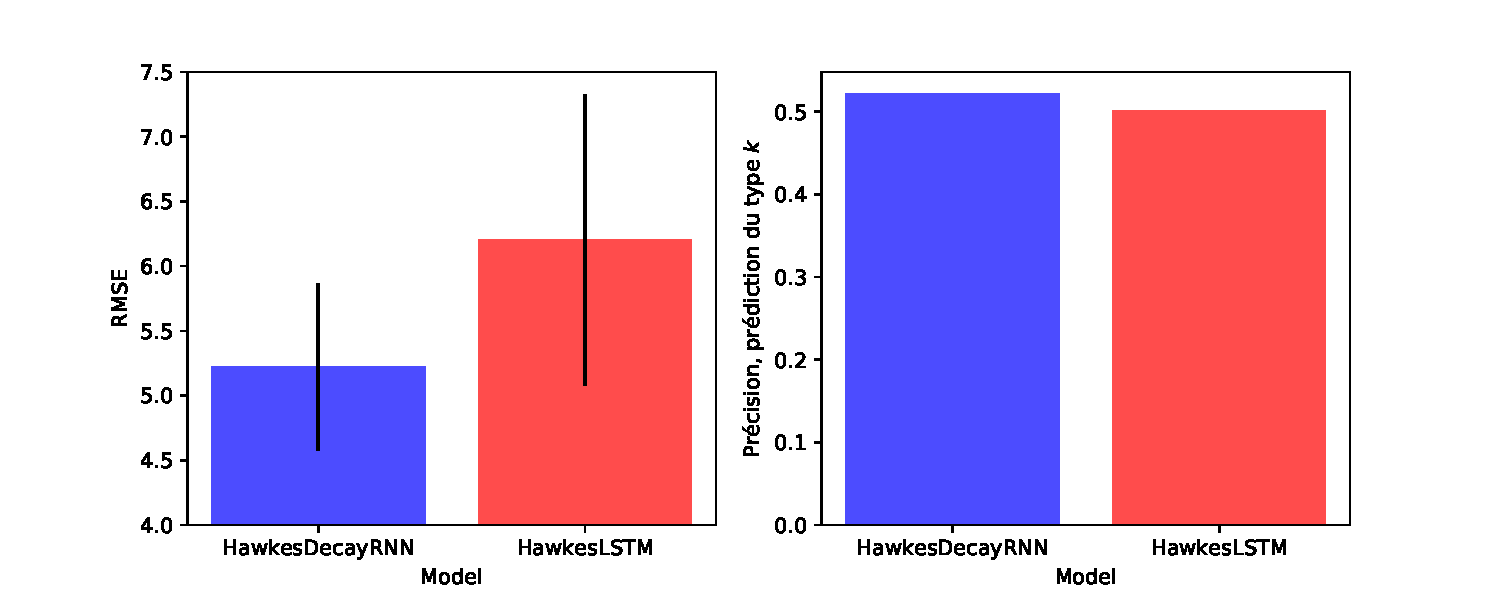
\includegraphics[width=\linewidth]{../results/2D_Hawkes_Data_RMSE.pdf}
		\caption{RMSE et précision de prédiction du type $k_i$, modèles Decay-RNN et LSTM. Données synthétiques Hawkes, $K=2$, $D=64$.}\label{fig:rmse2DhawkesData}	
	\end{subfigure}
	\caption{Erreur quadratique de prédiction pour les modèles Decay-RNN et LSTM.}\label{fig:rmseSynthData}
\end{figure}

La fonction de perte du modèle RMTPP ne semble pas converger au cours de son entraînement \autoref{fig:loss}, et ce malgré plusieurs ajustements (voir \eqref{eq:rmtppLambdaModified}) par rapport à \autocite{DuRMTPP}.
\begin{figure}[!ht]
	\centering
	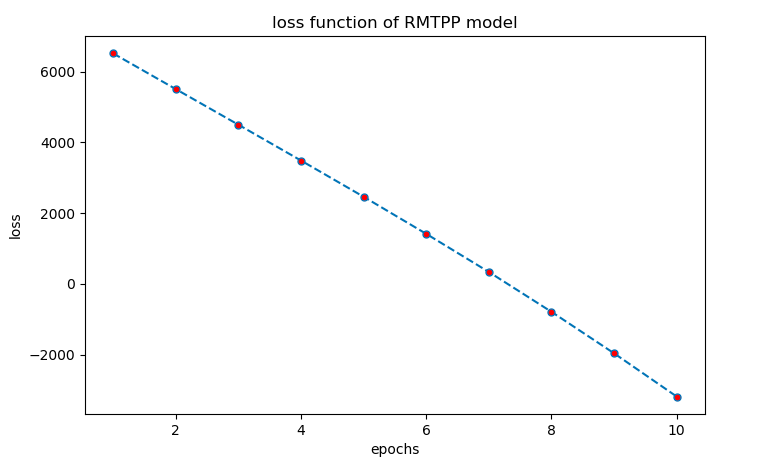
\includegraphics[width=\linewidth]{../results/loss_funct}
	\caption{Fonction de perte pour le modèle RMTPP, entraîné sur le jeu de données Hawkes bidimensionnel ($K=2$) \autoref{tab:synthHawkesData}.}\label{fig:loss}
\end{figure}


\end{document}